
\section{Implementation Issues}

While implementing HMM for both character recognition and word recognition, we encountered some practical issues.

\subsection{Initial Model Selection}
%4.1. Describe the different initialization algos, advantages and disadvantages. Chongyang


Hidden Markov models can be efficiently trained by Baum-Welch (BW) algorithm, which is an iterative process for estimating parameters for HMMs. 
As an iterative algorithm, BW starts from an initial model and estimates transition and emission probability parameters by computing expectations via the Forward-Backward algorithm.
The algorithm sums over all paths containing a given event until convergence is reached.

Since the Baum-Welch algorithm is a local iterative method, the resulting HMM and the number of required iterations depend heavily on the initial model. 
There are many ways to generate an initial model, some techniques consider the training data while others do not \cite{Laan}.
Similar to Laan et al. \cite{Laan}, we tried three initialization strategies,  count-based, random and uniform. % not sure what's meant by this: tested on the training data for character HMM model.

\subsection{Topology of HMM}

Because the EM algorithm assumes that the model is correct, it is important to devise a suitable topology before training starts. 
The topology of the model is usually built by using a prior knowledge of the data \cite{Suen}. 
For handwritten signals, a left-to-right HMM is often used where no back transitions from right to left are allowed.

\begin{enumerate}
\item	Character classifier: A model is created for each character in the training phase.

Because the English alphabet only contains 26 characters, it is not too computationally costly to train a separate model for each character.
We used special beginning and end states denoted by \textit{b} and \textit{e} respectively, similar to the model suggested by Laan et al. \cite{Laan}.
Special beginning and end states are included because multiple training observation sequences are concatenated to form one observation sequence.
The sequence is then used as input for the BW algorithm.

In the concatenated string, we also used special beginning and end observation symbols @ and \$.
The  beginning state   \textit{b} always transitions to the first normal state, and the  ending state \textit{e} always transitions back to \textit{b}.
Finally, the forward-backward algorithm is used to choose the model that has the most probability of generating the observation sequence. 
% TODO: Missing figure again
See \ref{figure:wordtopology}.

\begin{figure}[h!]
\centering
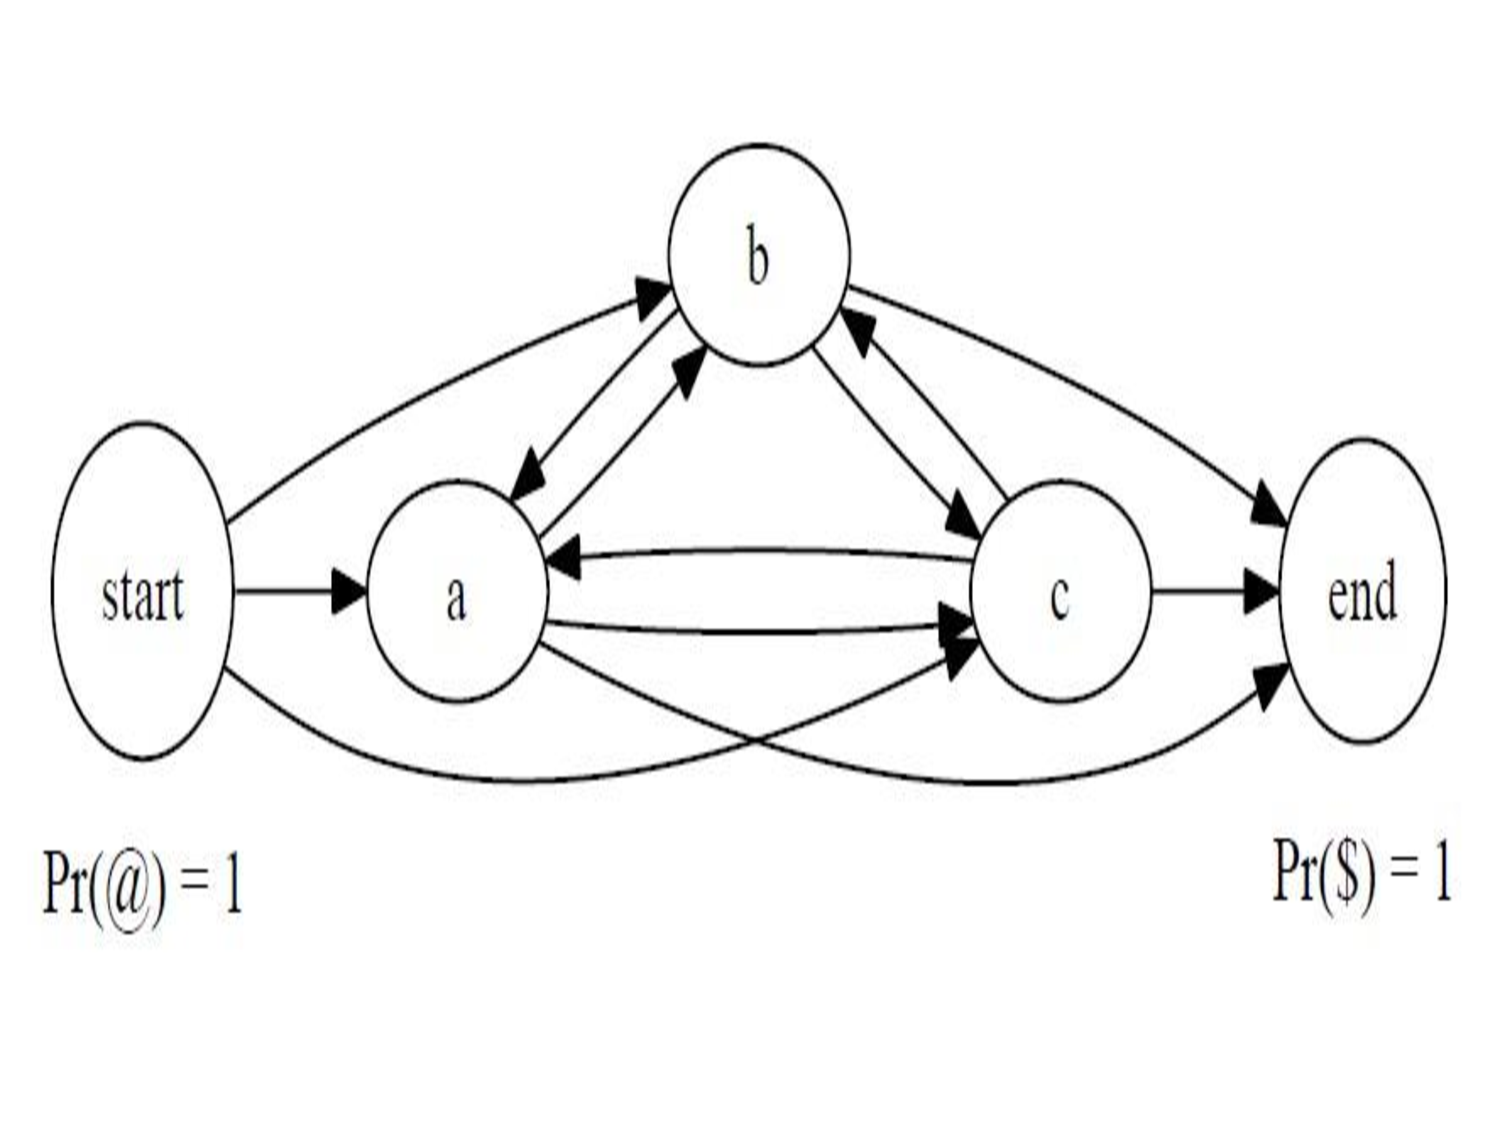
\includegraphics[width=5in]{wordtopology}
\caption{Word HMM topology for a three-letter alphabet.}
\label{figure:wordtopology}
\end{figure}


\item	Word classifier: A single model is constructed for the whole vocabulary. 

Generally it’s natural to implement Hidden Markov Models for each of the word when vocabulary is limited and small. And similar topologies can be found among those HMMs. Then we can also use forward and backward algorithm to choose the most likely model to tell which word it is as what we did for character classifier above. It works really well when we classify the test data to get the results within 20 words as following.

["dog","cat","pig","love","hate","scala","python","summer","winter",\\"night",daydream","nightmare","animal","happiness","sadness","tennis",\\"feminism","fascism","socialism","capitalism"]

However, it is time consuming and not realistic to generate HMMs for every word when the vocabulary is relatively large. Therefore, later on we came up with another HMM topology to ideally describe unconstrained words of mixed style.

To be specific, a Hmm  with a topology that is a complete directed graph is modeled. It has 28 hidden states(26 for 26 letters and 2 for @ and \$). 
Transition matrix is a 28 * 28 matrix, which is estimated from the lexicon analysis. For example if there's only three words in our vocabulary: dog cat cap for "A to T is set to 0.5 and A to P is set to 0.5" and "A to other letters is set to 0".

Each state's observation is the letter we observed from the character classifier in the previous step. For setting the observation probability matrix, it's reasonable to set them to the probabilities from the test results from word classifier. For example, if we have 10 test examples , for A and 5 of them are classified to be A, 3 to B and 2 to C by the character classifier, then P(observation A)=0.5, P(observation B)=0.3 and P(observation C)=0.2. Then we will assign the row for A as"0.5 0.3 0.2 0 0 ......0 0".

\end{enumerate}

\subsection{Floating Point Precision}

When the number of states \textbf{t} grows sufficiently large, the forward variable $\textbf{a}_t(i)$ and backward variable  $\textbf{b}_t(i)$  exponentially approaches zero and exceed the precision range of floating point numbers.
One way to solve this problem is by incorporating a scaling procedure.
For each \textbf{t}, we first compute $\textbf{a}_t(i)$ according to the induction equation (20) in  \cite{Rabiner1989}, and then multiply it by a scaling factor  $\textbf{c}_t$, calculated by Equation \ref{eq:rabiner-scaling}.
% Maybe we should the explain the equation in more detail.. For example what  N is.

\begin{equation}\label{eq:rabiner-scaling}
\textbf{c}_t = \frac{1}{ \displaystyle\sum_{i=1}^N \textbf{a}_t(i)}
\end{equation}

To avoid the underflow problem in the Viterbi algorithm, which calculates the maximum likelihood state sequence, we add log probabilities instead of multiplying probabilities.
With this change, no scaling is required.

\subsection{Zero Probability Transitions}
% We should explain WHY this is a problem.
Another problem that may occur when training HMM parameters is that state transition probabilities are likely to be zero.
In our implementation, we initialize them to a very small number, such as \textbf{ $10^{-10}$}.



